\documentclass[tikz,border=7pt]{standalone}

\usepackage{iftex}
\ifPDFTeX
  \PackageError{matrix-figure}{This figure requires XeTeX or Tectonic}{Compile with xelatex or tectonic.}
\fi
\usepackage{fontspec}
\usepackage{xeCJK}
\usepackage{amsmath}
\usepackage{unicode-math}
\usepackage{xcolor}
\usepackage{tikz}
\usetikzlibrary{positioning}

\providecommand{\FigureUseLocalFonts}{0}
\ifnum\FigureUseLocalFonts=1
  \setmainfont{NotoSansCJKtc-Regular.otf}[Path=\FigureSansFontPath]
  \setsansfont{NotoSansCJKtc-Regular.otf}[Path=\FigureSansFontPath,BoldFont=NotoSansCJKtc-Bold.otf]
  \setCJKmainfont{NotoSansCJKtc-Regular.otf}[Path=\FigureSansFontPath]
  \setCJKsansfont{NotoSansCJKtc-Regular.otf}[Path=\FigureSansFontPath,BoldFont=NotoSansCJKtc-Bold.otf]
  \setmathfont{STIXTwoMath.otf}[Path=\FigureMathFontPath]
\else
  \setmainfont{Noto Sans CJK TC}
  \setsansfont{Noto Sans CJK TC}
  \setCJKmainfont{Noto Sans CJK TC}
  \setCJKsansfont{Noto Sans CJK TC}
  \setmathfont{STIX Two Math}
\fi

\definecolor{FigureInk}{HTML}{253142}
\definecolor{PanelMiddle}{gray}{0.94}
\definecolor{PanelRight}{gray}{0.86}

\newcommand{\FigureAugMatrix}[1]{%
  \renewcommand{\arraystretch}{1.25}%
  \left[\begin{array}{ccc|c}#1\end{array}\right]%
}

\begin{document}
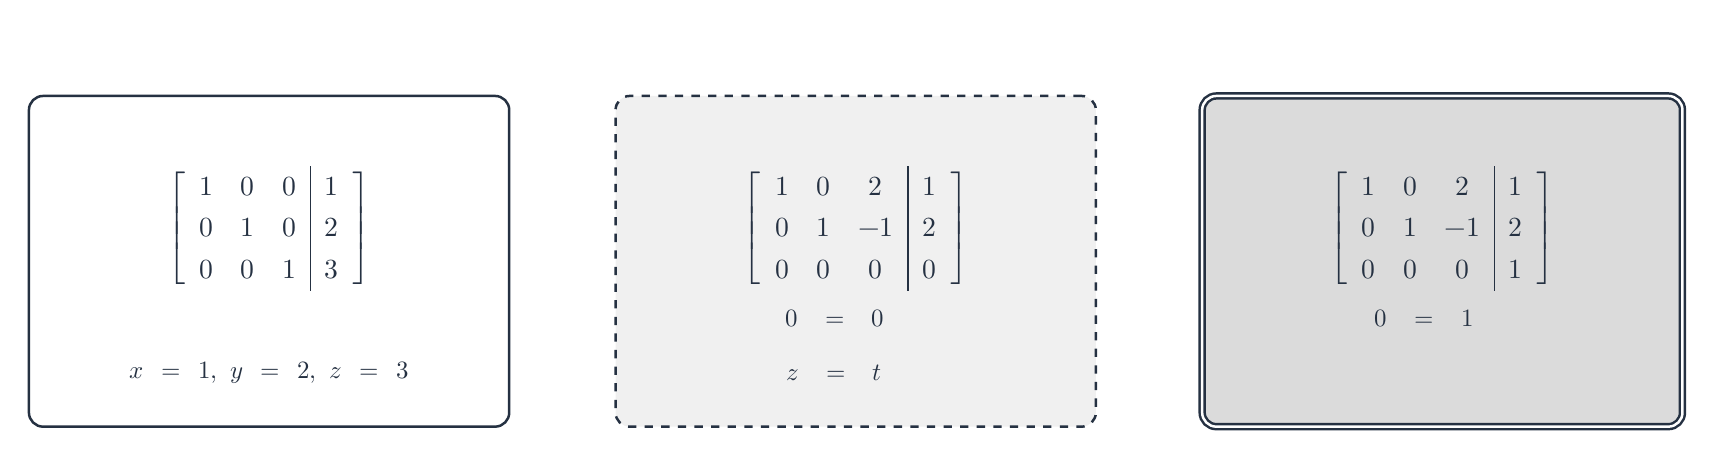
\begin{tikzpicture}[
  font=\sffamily,
  text=FigureInk,
  panel/.style={draw=FigureInk,line width=0.9pt,rounded corners=1.8mm,minimum width=6.1cm,minimum height=4.2cm,inner sep=9pt},
  heading/.style={font=\bfseries\large,align=center},
  reason/.style={font=\small,align=center,text width=5.5cm},
  conclusion/.style={font=\bfseries\small,align=center,text width=5.5cm},
]
  \node[font=\bfseries\Large,align=center,text width=20cm] at (10.3,5.60)
    {消去後最後一列與樞紐數量，直接決定方程組的解型};

  \node[panel,fill=white] (unique) at (2.85,2.75) {};
  \node[panel,fill=PanelMiddle,dashed] (infinite) at (10.30,2.75) {};
  \node[panel,fill=PanelRight,double,double distance=0.9pt] (none) at (17.75,2.75) {};

  \node[heading] at ([yshift=1.48cm]unique.center) {唯一解};
  \node at ([yshift=0.42cm]unique.center) {$
    \FigureAugMatrix{1&0&0&1\\0&1&0&2\\0&0&1&3}
  $};
  \node[reason] at ([yshift=-0.72cm]unique.center) {三個變數都有樞紐};
  \node[conclusion] at ([yshift=-1.42cm]unique.center) {$x=1,\ y=2,\ z=3$};

  \node[heading] at ([yshift=1.48cm]infinite.center) {無限多組解};
  \node at ([yshift=0.42cm]infinite.center) {$
    \FigureAugMatrix{1&0&2&1\\0&1&-1&2\\0&0&0&0}
  $};
  \node[reason] at ([yshift=-0.72cm]infinite.center) {$0=0$，少一個樞紐};
  \node[conclusion] at ([yshift=-1.42cm]infinite.center) {$z=t$ 為自由變數};

  \node[heading] at ([yshift=1.48cm]none.center) {無解};
  \node at ([yshift=0.42cm]none.center) {$
    \FigureAugMatrix{1&0&2&1\\0&1&-1&2\\0&0&0&1}
  $};
  \node[reason] at ([yshift=-0.72cm]none.center) {$0=1$ 形成矛盾};
  \node[conclusion] at ([yshift=-1.42cm]none.center) {方程組不相容};
\end{tikzpicture}
\end{document}
